\iffalse
\let\negmedspace\undefined
\let\negthickspace\undefined
\documentclass[journal,12pt,twocolumn]{IEEEtran}
\usepackage{cite}
\usepackage{amsmath,amssymb,amsfonts,amsthm}
\usepackage{algorithmic}
\usepackage{graphicx}
\usepackage{textcomp}
\usepackage{xcolor}
\usepackage{txfonts}
\usepackage{listings}
\usepackage{enumitem}
\usepackage{mathtools}
\usepackage{gensymb}
\usepackage{comment}
\usepackage[breaklinks=true]{hyperref}
\usepackage{tkz-euclide} 
\use-package{listings}
\usepackage{gvv}                                        
\def\inputGnumericTable{}                                 
\usepackage[latin1]{inputenc}                                
\usepackage{color}                                            
\usepackage{array}                                            
\usepackage{longtable}                                       
\usepackage{calc}                                             
\usepackage{multirow}                                         
\usepackage{hhline}                                           
\usepackage{ifthen}                                           
\usepackage{lscape}
\usepackage{caption}

\newtheorem{theorem}{Theorem}[section]
\newtheorem{problem}{Problem}
\newtheorem{proposition}{Proposition}[section]
\newtheorem{lemma}{Lemma}[section]
\newtheorem{corollary}[theorem]{Corollary}
\newtheorem{example}{Example}[section]
\newtheorem{definition}[problem]{Definition}
\newcommand{\BEQA}{\begin{eqnarray}}
\newcommand{\EEQA}{\end{eqnarray}}
\newcommand{\define}{\stackrel{\triangle}{=}}
\theoremstyle{remark}
\newtheorem{rem}{Remark}
\begin{document}

\bibliographystyle{IEEEtran}
\vspace{3cm}

\title{11.9.5}
\author{EE23BTECH11029 - Kanishk}
\maketitle

\bigskip


\textbf{Question}:\\ 
The sum of the first four terms of an A.P. is 56. The sum of the last four terms is
112. If its first term is 11, then find the number of terms.\\

\textbf{Solution}:\\ 
\fi
\begin{table}[ht]
    \centering
    \def\arraystretch{1.5}
    \footnotesize
\begin{tabular}{|c|c|c|}
\hline
Symbol & Value & Description\\
\hline
$x(0)$ & $11$ & First term of AP \\
\hline
$y\brak{3}$ & $56$ & Sum of the first four terms of AP\\
\hline
$y\brak{n}-y\brak{n-4}$ & $112$& Sum of the last four terms of AP\\
\hline
\end{tabular}

   \caption{Input Parameters}
   \label{tab:11.9.5.12}
\end{table}

\small
\begin{align}
y\brak{n}&=\sbrak{\frac{\brak{n+1}}{2}\brak{2x\brak{0}+nd}}u\brak{n}\\
\implies y(3)&=\frac{4}{2}\brak{2x\brak{0}+3d}\\
\end{align}
From \tabref{tab:11.9.5.12}:
\begin{align}
\frac{4}{2}\brak{2x\brak{0}+3d}&=56\\
2x\brak{0}+3d&=28\\
\implies d&=2
\end{align}

\begin{align}
 y\brak{n}-y\brak{n-4}&=\frac{4}{2}\brak{2x\brak{n}+3\brak{-d}}
\end{align}
From \tabref{tab:11.9.5.12}:
\begin{align}
\frac{4}{2}\brak{2x\brak{n}+3\brak{-d}}&=112\\
2x\brak{n}-3d&=56\\
\implies x\brak{n}&=31\\
x\brak{0}+\brak{n}2&=31\\
\implies n&=10
\end{align}


\begin{align}
x\brak{n}&=\brak{x\brak{0}+2n}u\brak{n}\\
\implies X\brak{z}&=\frac{x\brak{0}}{1-z^{-1}}+2\frac{z^{-1}}{\brak{1-z^{-1}}^{2}}.\quad \abs{z} > 1
\end{align}

\newpage

\begin{figure}
    
    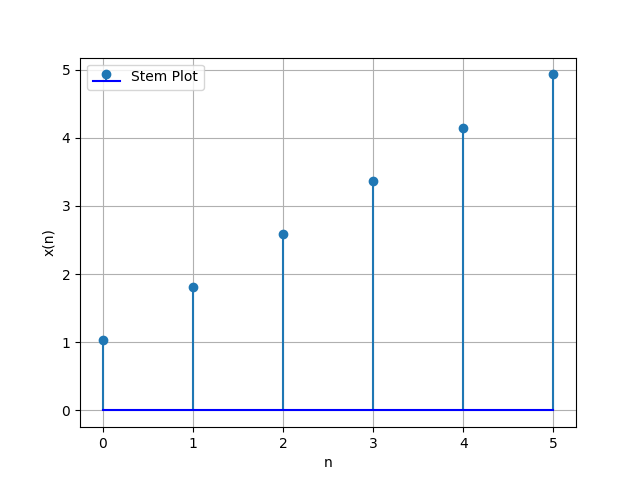
\includegraphics[width=\columnwidth]{ncert-maths/11/9/5/12//figs/fig1.png}
    \caption{Plot y(n) vs n}
\end{figure}

%\end{document}